\documentclass[12pt,conference,a4paper,twocolumn]{IEEEtran}
\usepackage[left=2cm,right=2cm,top=2cm,bottom=2cm]{geometry}
\usepackage[utf8]{inputenc}
\usepackage[english]{babel}

\usepackage{amsmath}
\usepackage{amsfonts}
\usepackage{amssymb}
\usepackage{graphicx}
\usepackage{listings}
\usepackage{cite}
\usepackage{hyperref}
\hypersetup{colorlinks=false,linktoc=all,linkcolor=blue}
\usepackage{textcomp}
\usepackage{xcolor}
\usepackage{algorithmic}

\definecolor{mygrey}{gray}{0.97}
\lstset{
  basicstyle=\tiny,
  columns=fullflexible,
  breaklines=true,
  postbreak=\mbox{{$\hookrightarrow$}\space},
  backgroundcolor=\color{mygrey},
  numbers=left,
  xleftmargin=3em,
  framexleftmargin=3em,
  %frame=single,
  %language=Matlab, 
  tabsize=3,
  escapeinside={\%latex}{\%latex},
}


\title{Control and Instrumentation Laboratory (EC692)\\Experiment No.: 2}
\author{	\IEEEauthorblockN{Dhiman Sarkar}
			\IEEEauthorblockA{\\
							Roll: 19101105086\\
							Dept. of Electronics and Comm. Engineering\\
							Jalpaiguri Government Engineering College\\
							Email: ds2286@ece.jgec.ac.in
							}
			\and
			\IEEEauthorblockN{Alok Barman}
			\IEEEauthorblockA{\\
							Roll: 19101105087\\
							Dept. of Electronics and Comm. Engineering\\
							Jalpaiguri Government Engineering College\\
							Email: ab2287@ece.jgec.ac.in
							}
			\and
			\IEEEauthorblockN{Alka Tigga}
			\IEEEauthorblockA{\\
							Roll: 19101105088\\
							Dept. of Electronics and Comm. Engineering\\
							Jalpaiguri Government Engineering College\\
							Email: at2288@ece.jgec.ac.in
							}
			\and
			\IEEEauthorblockN{Azizul Mallick}
			\IEEEauthorblockA{\\
							Roll: 19101105089\\
							Dept. of Electronics and Comm. Engineering\\
							Jalpaiguri Government Engineering College\\
							Email: am2289@ece.jgec.ac.in
							}
		}

\begin{document}
\maketitle
\begin{abstract}
	Familiarization with MATLAB and generation of various types of signals.
\end{abstract}

\section{Brief Description of The Experiment}
\begin{enumerate}
\item[a)] Generation of the following signals and their plots plot in MATLAB
	\begin{enumerate}
	\item[i)] a unit impulse at t=0, 
	\item[ii)] a unit step, 
	\item[iii)] a ramp, 
	\item[iv)] an aperiodic pulse of duration 0.25 ms
	\end{enumerate}
\item[b)] Generation and plot of a square wave with period 0.5s and amplitude 0.81.
\item[c)] Generation of a delayed versions of the signals generated in the previous problem. Delay time = 2ms.
\item[d)] Generation of the following signals,
	\begin{enumerate}
	\item[i)] An impulse train with period 1ms.
	\item[ii)] A pulse train with period 1ms and a duty cycle of (i) 0.25, (ii) 0.5. Plot atleast 10 cycles.
	\end{enumerate}
\end{enumerate}

\section{MATLAB Scripts}
Exercise - 1
\lstinputlisting[firstline=3,name=MATLAB]{exc1.m}
Exercise - 2
\lstinputlisting[firstline=3,name=MATLAB]{exc2.m}
Exercise - 3
\lstinputlisting[firstline=3,name=MATLAB]{exc3.m}
Exercise - 4
\lstinputlisting[firstline=3,name=MATLAB]{exc4.m}

\section{Output Results and Plots}

\begin{figure}[h]
\centering
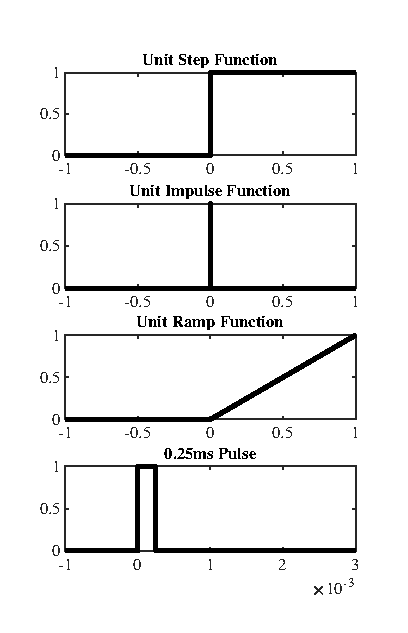
\includegraphics[width=2.5in]{exc1.eps}
\caption{Plot of various signals specified in Exercise 1}
\end{figure}

\begin{figure}[ht]
\centering
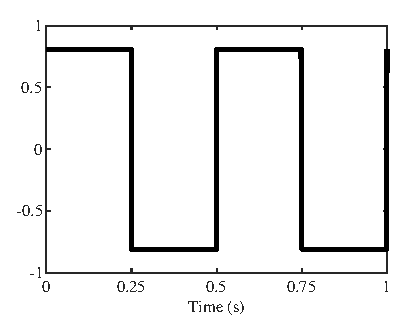
\includegraphics[width=2.5in]{exc2.eps}
\caption{Plot of Exercise-2}
\end{figure}

\begin{figure}[h!]
\centering
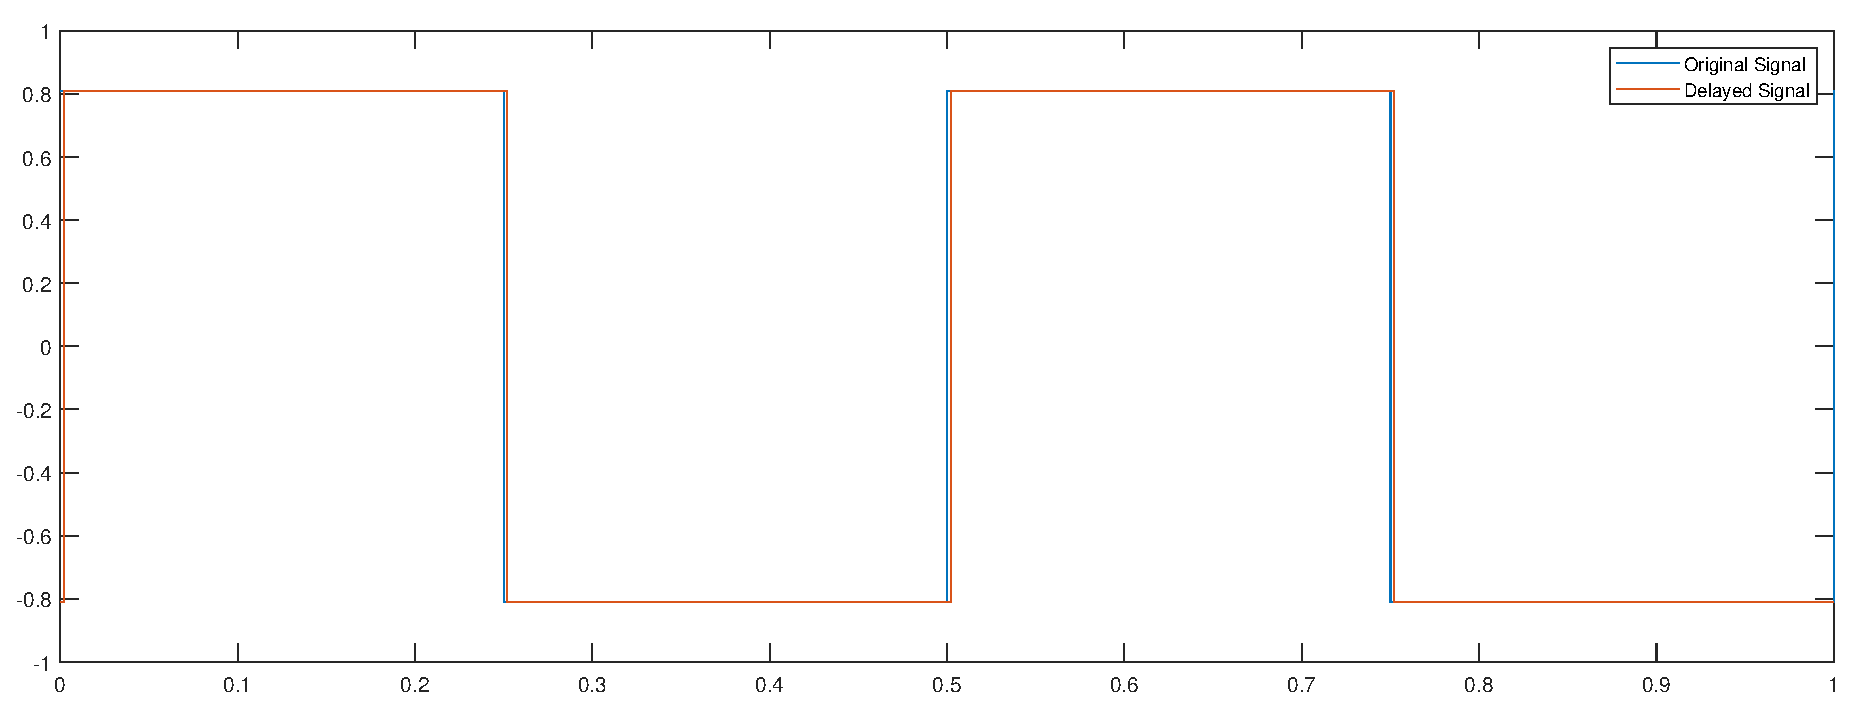
\includegraphics[width=2.5in]{exc3_1.eps}
\caption{Plot of a delayed signal}
\label{delay_signal}
\end{figure}

\begin{figure}[h!]
\centering
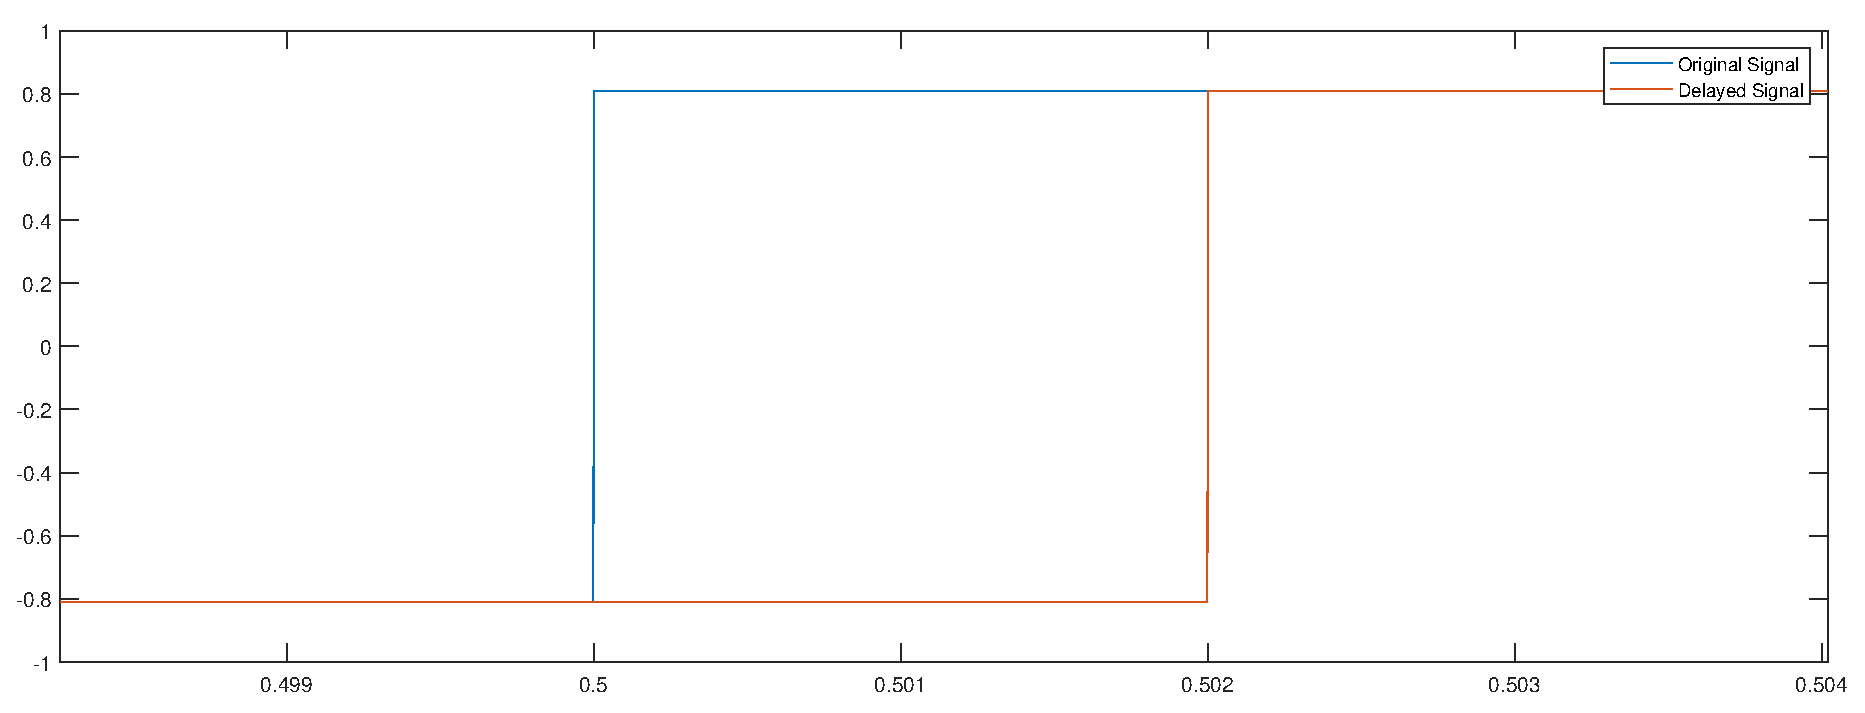
\includegraphics[width=2.5in]{exc3_2.eps}
\caption{A close inspecection around 0.5s of Fig.\ref{delay_signal}}
\end{figure}

\begin{figure}[h!]
\centering
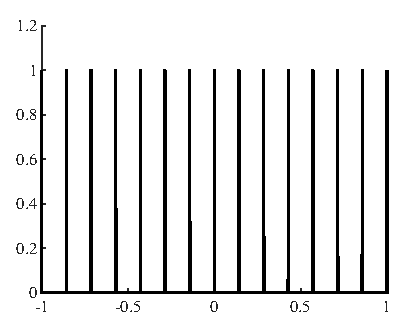
\includegraphics[width=2.5in]{exc4_a.eps}
\caption{Plot impulse train specified in Exercise 4(i)}
\end{figure}

\begin{figure}[h!]
\centering
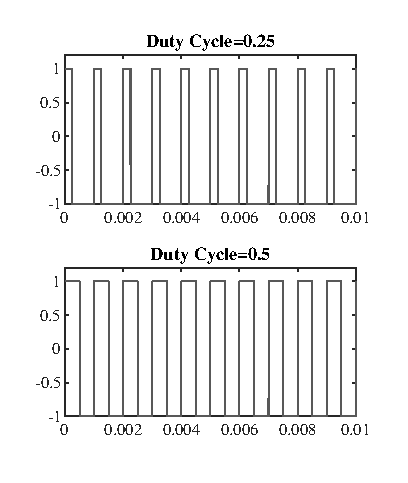
\includegraphics[width=2.5in]{exc4_b.eps}
\caption{Plot of two suare waves of same period but different Duty Cycle specified in Exercise 4(ii)}
\end{figure}


\section{Observations \& Conclusion}
Test signals are always a useful tool in analysis of a system. Previously we've learned to analyze systems in both Time-Domain and Frequency-Domain analytically. And now that we have learned how to generate the test signals in MATLAB, it'll be helpful for analyzing systems numerically. 

\section{Acknowledgment}
We would like to express our sincere gratitude to our course instructor Mr. Mirwaiz Rahaman and Mrs. Purba Basu for providing their invaluable guidance, comments and suggestions.

\end{document}